%!TEX root = ./slopecd.tex

\section{Theory}\label{sec:theory}
%%%%%%%%%%%%%%%%%%%%%%%%%%%%%%%%%%%%

\subsection{Coordinate Descent for SLOPE}%
\label{sec:coordinate-updates}

In this section we derive a coordinate descent algorithm for minimizing the SLOPE problem~\eqref{eq:slope-problem} with respect to the coefficients of a single cluster at a time.
First observe that we can write \eqref{eq:slope-problem}.
\[
  \begin{aligned}
    P(\beta) & =  \frac{1}{2} \lVert y - X\beta\rVert_2^2 + J(\beta)                                                                                                                                                                                                                \\
             & = \frac{1}{2} \lVert y - X_{\bar{\mathcal{C}_k}} \beta_{\bar{\mathcal{C}_k}} - \big(X_{\mathcal{C}_k} s_{\mathcal{C}_k}\big)c_k  \rVert_2^2 + \sum_{j \notin {\mathcal{C}_k}} \lambda_{(j)^-}|\beta_k| + \bigg(\sum_{j \in {\mathcal{C}_k}} \lambda_{(j)^-}\bigg)c_k \\
             & = \frac{1}{2} \lVert \tilde r - \tilde x c_k \rVert_2^2 + \sum_{j \notin {\mathcal{C}_k}} \lambda_{(j)^-}|\beta_k| + \bigg(\sum_{j \in {\mathcal{C}_k}} \lambda_{(j)^-}\bigg)c_k                                                                                     \\
  \end{aligned}
\]
with \( \tilde x_k = X_{\mathcal{C}_k} s_{\mathcal{C}_k}\) and
where \(\tilde r_k = y - \tilde y_k = y - X_{\bar{\mathcal{C}}_k} \beta_{\bar{\mathcal{C}_k}}\).

Our coordinate-wise update is based on optimizing over clusters' corresponding coefficients one at a time, keeping the relative signs of the coefficients inside each cluster constant, but allowing the signs of all of them to flip. This one-dimensional sub-problem is given by
\begin{equation*}
  \operatorname*{minimize}_{\alpha \in \mathbb{R}} \left( \frac{1}{2} \lVert \tilde r - \tilde x \alpha_k \rVert_2^2 + \sum_{j \notin {\mathcal{C}_k}} \lambda_{(j)^-}|\beta_k| + \bigg(\sum_{j \in {\mathcal{C}_k}} \lambda_{(j)^-}\bigg)|\alpha_k|\right).
\end{equation*}
Differentiating with respect to \(\alpha_k\), yields
\begin{equation}
  \label{eq:cluster-grad}
  \partial_{\alpha_k}
  P(\beta) = \tilde x^T \tilde x \alpha_k - \tilde r^T \tilde x +
  \partial_{\alpha_k} \Bigg(\sum_{j \notin \mathcal{C}_k}\lambda_{(j)^-}
  |\beta_j| + \bigg(\sum_{j \in {\mathcal{C}_k}} \lambda_{(j)^-}\bigg)|\alpha_k|
  \Bigg),
\end{equation}
where the last term is the partial subdifferential of the sorted \(\ell_1\)
norm.

\subsubsection{Naive Updates}

As in \textcite{friedman2010}, we can improve the efficiency of updates by observing that
\begin{equation}
  \begin{aligned}
    \tilde r_k & = y - \tilde y_k                                                     \\
               & = \underbrace{y - X_{\bar{\mathcal{C}_k}}\beta_{\bar{\mathcal{C}_k}}
    - \tilde x c_k}_r + \tilde x c_k                                                  \\
               & = r + \tilde x c_k.
  \end{aligned}
\end{equation}

\subsubsection{Storing Reductions}

Observe that \(\tilde x_k\) only changes between subsequent coordinate updates provided that the members of the cluster \(k\) change, for instance if two clusters are merged, a predictor leaves a cluster, or the signs flip (through an update of \(\alpha_k\)).
It is therefore possible to obtain significant computational gains by storing \(\tilde x_k\) and \(\tilde x_k^T \tilde x_k\) for each cluster. When there is no change in the clusters, we avoid these costly computations. And even when there are changes, we can still reduce the costs involved since \(\tilde x_k\) can be updated in place.

Letting \(\tilde x_k^\text{old}\) correspond to the value of \(\tilde x_k\) before the update, we note that
\(\tilde x_k \gets \tilde x_k^\text{old} + x_j \sign(\beta_j)\)
for each \(j \in \mathcal{C}_k^\text{new} \setminus \mathcal{C}_k^\text{old}\)
and \(\tilde x_k \gets \tilde x_k^\text{old} - x_j \sign(\beta_j)\) for each
\(j \in \mathcal{C}_k^\text{old} \setminus \mathcal{C}_k^\text{new}\). 
If instead only the signs flip, we simply have to also flip the signs in \(\tilde x_k\).


\subsubsection{Alternative Formulation}

An alternative formulation (with identical solution) is to minimize
\[
  \begin{aligned}
    P(c_k) & = \frac{1}{2} \lVert y - X_{\bar{\mathcal{C}_k}} \beta_{\bar{\mathcal{C}_k}} - \big(X_{\mathcal{C}_k} \beta_{\mathcal{C}_k}\big)c_k  \rVert_2^2 + \sum_{j \notin {\mathcal{C}_k}} \lambda_{(j)^-}|\beta_k| + |c_k|\bigg(\sum_{j \in {\mathcal{C}_k}} \lambda_{(j)^- }|\beta_j|\bigg),
  \end{aligned}
\]
and \(\beta_k := c_k\beta_k\).

\subsubsection{Partial Subdifferential of the Sorted \(\ell_1\) Norm}

We now derive a closed form expression for the subdifferential
of the sorted \(\ell_1\) norm.
\begin{theorem}
  \label{thm:cluster-subdifferential}
  The partial subdifferential for the sorted \(\ell_1\) norm with respect
  to \(\alpha_k\), is
  \[
    \partial_{\tilde \beta_k}  J(\beta)       =
    \begin{cases}
      \big[-\sum_{j=1}^{|C(0)|}\lambda^{C(0)}_j, \sum_{j=1}^{|C(0)|}\lambda^{C(0)}_j\big]                                                                        & \text{if } \alpha = 0,           \\
      \big[\sum_{j=|\mathcal{C}_i| - |\mathcal{C}_k|+1}^{|\mathcal{C}_i|}\lambda^{\mathcal{C}_i}_j, \sum_{j=1}^{|\mathcal{C}_k|}\lambda^{\mathcal{C}_i}_j\big]   & \text{if } \alpha = c_i \neq 0,  \\
      \big[-\sum_{j=1}^{|\mathcal{C}_k|}\lambda^{\mathcal{C}_i}_j, -\sum_{j=|\mathcal{C}_i| - |\mathcal{C}_k|+1}^{|\mathcal{C}_i|}\lambda^{\mathcal{C}_k}_j\big] & \text{if } \alpha = -c_i \neq 0, \\
      \{\sign(\alpha)\boldsymbol{1}^T\lambda^{C(\alpha)}\}                                                                                                       & \text{otherwise.
      }
      % \{\sign(\alpha) S\big(C(\alpha)\big)\}                                                                                                & \text{if } \alpha \neq c_i \neq 0, \\
      % [-S(\mathcal{C}_m), S(\mathcal{C}_m)]                                                                                                           & \text{if } \alpha = 0,             \\
      % [\sign(\alpha)S\big( C(c_i - \sign(\alpha)\varepsilon_i)\big), \sign(\alpha)S\big(C(c_i + \sign(\alpha)\varepsilon_i)\big)] & \text{if } |\alpha| = c_i,
    \end{cases}
  \]
\end{theorem}
\begin{proof}
  Consider a fixed \(\beta\) and set \(\beta_{\mathcal{C}_k}= s_{\mathcal{C}_k}x\).
  Now let us consider the function  \(f(x) = |x|\sum_{j \in \mathcal{C}_k}\lambda^x_{(j)^-} + \sum_{j \notin \mathcal{C}_k} \lambda^x_{(j)^-}|\beta_j|\), where the ordering of \(\lambda^x\) is with respect to the vector
  \[
    \beta(x)_k = \begin{cases}
      |x|       & \text{if } \mbox{\(k \in \mathcal{C}_k\)}, \\
      |\beta_k| & \mbox{otherwise}.
    \end{cases}
  \]
  .\mathurin{If \(f\) is only a function of \(\tilde \beta\), then the second term is constant, and since we are interested in subgradients, we should able to omit it?} \jonas{I added the notation so that it is clear that ordering of the \(\lambda\) depends on \(x\), hence we can not remove the second component.}
  \(g\in \mathbb{R} \) \mm{\(f/g\) > \(u\) or \(v\) for subgradient?} is a subgradient of \(f\) at \(x\) if
  \begin{equation}
    \label{eq:subgrad-ineq}
    f(x^*)=|x^*|\sum_{j \in C_k}\lambda^{x^*}_{(j)^-} + \sum_{j \notin C(x^*)}\lambda ^{x^*}_{(j)^-}|\beta_j|
    \geq f(x)+ g(x^* - x)=|x|\sum_{j \in C_k} \lambda^x_{(j)^-} + \sum_{j \notin C_k}\lambda^x_{(j)^-}|\beta^x_j| + g(x^* - x)
  \end{equation}
  for all \(x^* \in \mathbb{R}\).
  Without loss of generality, since \(f\) is convex \mathurin{here I did not understand the WLOG relationship with convexity}, assume that we have
  a vector \(\beta\) such that there are two clusters: one corresponding
  to \(\alpha\), which we are optimizing over, and
  one additional cluster \(\mathcal{C}_q\) with corresponding
  coefficient \(c_q\).
  Then we can rewrite \eqref{eq:subgrad-ineq} as
  \[
    |y|S\big(C(y)\big) + c_q S\big(\widebar{C(y)}\big) \geq
    |x| S\big(C(x)\big) + c_q S\big(\widebar{C(x)}\big) + g(y - x).
  \]
  First observe that any \(g\) is permissible whenever \(x = y\).

  At \(x = 0\), \eqref{eq:subgrad-ineq} reduces to
  \[
    |y|S\big(C(y)\big) + c_q S\big(\widebar{C(y)}\big)
    \geq c_q S(\mathcal{C}_1) + gy.
  \]
  Because \(f\) is convex, it is sufficient to consider \(|y| < c_q\),
  in which case \(C(y) = \mathcal{C}_1\) and hence
  \begin{equation}
    |y|S(\mathcal{C}_2) + c_q S(\mathcal{C}_1) \geq c_q S(\mathcal{C}_1) + gy \implies
    |y|S(\mathcal{C}_2) \geq gy,
  \end{equation}
  which means that \(-S(\mathcal{C}_2) \leq g \leq S(\mathcal{C}_2)\).

  If \(x = c_q\), \eqref{eq:subgrad-ineq} becomes
  \[
    |y|S\big(C(y)\big) + x S\big(C(x)\big) \geq x(S(\mathcal{C}_1) + S(\mathcal{C}_2)) + g(y - x).
  \]
  For \(y > x\) we have \(C(y) = \mathcal{C}_1\) and consequently
  \[
    y\big(S(\mathcal{C}_1) - g\big) + x\big(g - S(\mathcal{C}_1)\big) \geq 0,
  \]
  which means that \(g \leq S(\mathcal{C}_1)\).
  Then, for \(0 < y < x\), we see
  \[
    y\big(S(\mathcal{C}_2) - g\big) + x(g - S(\mathcal{C}_2)\big) \geq 0,
  \]
  and hence \(g \geq S(\mathcal{C}_2)\).
  Using the same argument for \(x = -c_q\), we find that we in this case
  must have \(g\) such that
  \(-S(\mathcal{C}_1) \geq g \geq - S(\mathcal{C}_2)\).
  For all other choices of \(x\), \(f\) is differentiable with
  derivative \(\sign(\alpha)S\big(C(\alpha)\big)\).
\end{proof}

The objective and subgradient for the cluster-wise problem are shown in
\cref{fig:cluster-grad-obj}.

\begin{figure}[htbp]
  \centering
  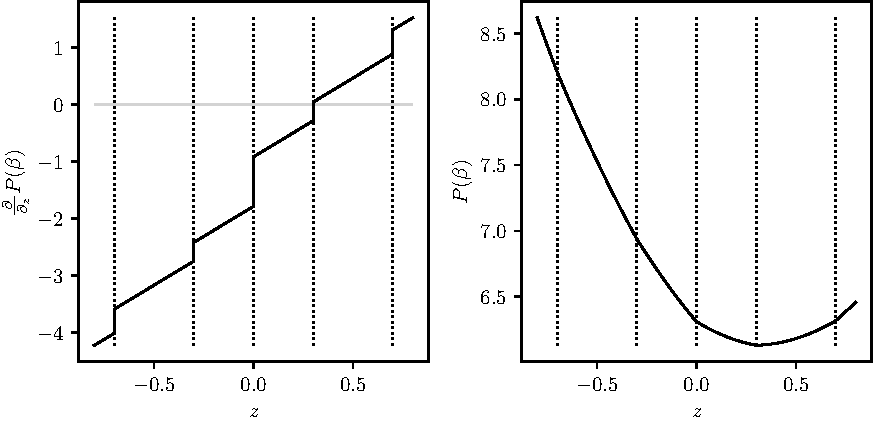
\includegraphics[]{clusterupdate-grad-obj}
  \caption{%
    Objective and gradient under the constraint that we have a fixed
    cluster.
    The optimum is found at \(\alpha = 0.3\).
  }%
  \label{fig:cluster-grad-obj}
\end{figure}

Let \(\mathcal{B}\) be a cluster initialized to \(\mathcal{C}_k\), with
corresponding coefficient \(c_k\).
Then the coordinate update for \(\beta_\mathcal{B}\) is\jl{This obviously
  does not work when \(s=0\). Can we just set \(s = 1\) here? It's just
  the relative signs that really matter, right?}\jw{That is a really good point. Do you think we can tie to the sign of the gradient instead?. We also will not move the zero cluster this way suspect. But it should work for any formation then sign of the gradient is the way I think?}
\jl{Yes, I think you're right, in fact that's what I have in the code now.}
\[
  \beta_\mathcal{B} \gets
  s_\mathcal{B}
  T \left(
  \frac{\tilde r^T \tilde x}{\tilde x^T \tilde x},
  \frac{\lambda}{\tilde x^T \tilde x},
  k,
  \tilde \beta,
  \mathcal{C}
  \right)
\]
where

\begin{equation}
  \label{eq:slope-thresholding}
  T(a, \lambda,k,\tilde \beta, \mathcal{C}) =
  \begin{cases}
    0                                                                 & \text{if } |a| \leq \sum_{i=1}^{|\mathcal{C}_k|}\lambda^{C_0}_i                                                                                                                               \\
    \sign(a)|\tilde \beta_i|                                          & \text{if } \sum_{j= |\mathcal{C}_i| - |\mathcal{C}_k| + 1}^{|\mathcal{C}_i|} \lambda^{\mathcal{C}_i}_j \leq |a| - |\tilde \beta_i| \leq \sum_{j=1}^{|\mathcal{C}_k|}\lambda^{\mathcal{C}_i}_j \\
    \sign(a)\big(|a| - \sum_{j \in \mathcal{C}_k}\lambda_{(j)^-}\big) & \text{otherwise.
    }
  \end{cases}
\end{equation}
To emphasize the connection between \(T\) and the soft-thresholding operator
for the lasso, we call this operator the SLOPE-thresholding operator.
In \cref{fig:slope-thresholding}, we visualize the operator.

\begin{figure}[htbp]
  \centering
  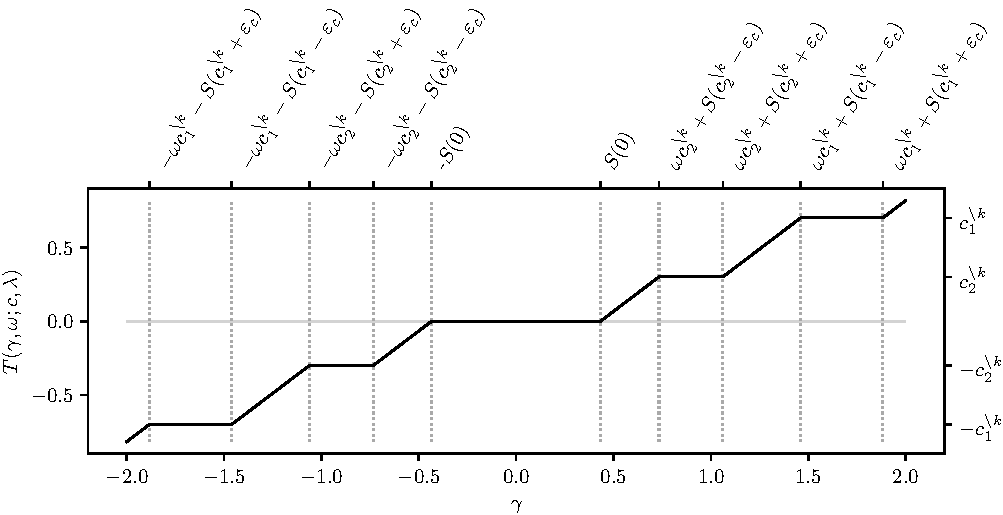
\includegraphics[]{slope-thresholding.pdf}
  \caption{The result of the SLOPE thresholding update.}
  \label{fig:slope-thresholding}
\end{figure}

\subsection{Hybrid proximal coordinate descent strategy}

We propose an iterative solver that alternates between proximal gradient step and proximal coordinate descent.
Since the regularization term for SLOPE is not separable, applying PCD does not guarantee convergence (show example where CD gets stuck).
However, \cite{dupuis2021} showed that once the clusters are known, the subdifferential of $J$ can be written as the cartesian product of the subdifferential of $J$ restricted to the clusters. 
Hence, if one knew the clusters, PCD updates could be applied on each cluster. 

The notion of clusters for SLOPE extends the notion of sparsity coming from the LASSO. 
Identification of the sparsity pattern throughout the iterative algorithm have largely been studied. 
Talk about Partly Smooth functions, related Manifold and that support transpose to cluster for SLOPE regularization. DO the maths. 

Then identification of this underlying structure occurs when applying PGD. 
Hence the idea to alternate, PGD and PCD step to take advantage of the speed of PCD and ensure convergence via the identification of the right structure with PGD steps. 

\begin{algorithm}[tb]
  \SetKwInOut{Init}{init}
  \SetKwInOut{Input}{input}
  \caption{%
    Hybrid coordinate descent and proximal gradient descent algorithm
    for SLOPE\label{alg:hybrid}}
  \Input{
    \(X \in \mathbb{R}^{n\times p}, y\in \mathbb{R}^n, \beta\in \mathbb{R}^p, \lambda \in \{\mathbb{R}^p : \lambda_1 \geq \lambda_2 \geq \cdots > 0\}\), \(m \in \mathbb{N}\)}

  \Init{\(t \gets 0\), \(\beta \gets 0\), \(L \gets \lVert X \rVert_2^2\)}

  \Repeat{convergence}{
  \(t \gets t + 1\)

  \If{\(t \bmod m = 0\)}{

  \(\beta \leftarrow \operatorname{prox}_{J / L}(\beta - \frac{1}{L}\nabla f(\beta))\) \label{alg:hybrid-istastep}

  % \(C_1, \hdots, C_m \leftarrow \mathtt{get\_clusters}(\beta)\)
  }
  \Else{
    \(k \gets 0\)

    \While{\(k \leq \lvert \mathcal{C} \rvert\)}{
      \(k \gets k + 1\)

      \(s \leftarrow \mathrm{sign}(\beta_{\mathcal{C}_k})\)

      \If{\(s \neq 0\)}{
        % \(L_k \gets (X_{:, \mathcal{C}_k}s)^\top  X_{:, \mathcal{C}_k}s\)


        % \(\tilde{\beta} \gets T(|\beta_{\mathcal{C}_k}| - \frac{1}{L_k} \nabla_{\mathcal{C}_k}f(\beta)^\top s, \frac{\lambda}{L_k})\)

        % \(\beta_{\mathcal{C}_k} \leftarrow \tilde{\beta} s\)
        \(\tilde x_k \gets X_{\mathcal{C}_k}s\)

        \(\tilde y_k \gets X_{\widebar{\mathcal{C}}_k}\beta_{\widebar{\mathcal{C}}_k}\)

        \(\tilde r_k \gets y - \tilde y_k\)

        \(
        \beta_{\mathcal{C}_k} \gets
        s T \left(
        \frac{\tilde r^T_k \tilde x_k, }{ \tilde x_k^T \tilde x_k},
        \frac{\lambda}{ \tilde x_k^T \tilde x_k},
        k,
        \tilde \beta,
        \mathcal{C}
        \right)
        \)
        \Comment{\(\mathcal{C}\) is updated at this step.}


      }

    }
  }

  }
  \Return{\(\beta\)}
\end{algorithm}

\begin{theorem}
  Iterates of \cref{alg:hybrid} converge towards \(\beta^*\).
\end{theorem}
\begin{proof}
  First note that convergence properties of proximal gradient descent on convex
  problems such as SLOPE are well-established
  \parencite{beck2009,daubechies2004}, which certifies that updates via
  \cref{alg:hybrid-istastep} make progress towards \(\beta^*\).

  Next note that the objectives of \eqref{eq:slope-problem} and
  \eqref{eq:subproblem} are equal and that \eqref{eq:subproblem} can be seen
  viewed as a version of \eqref{eq:slope-problem} with added linear constraints
  that is also convex. And, finally, because the coordinate updates of
  \cref{alg:hybrid} minimize the sub-problem, we in the worst case make no
  progress and therefore have guaranteed converge rate no less than \(1/m\)
  of that of proximal gradient descent.
\end{proof}

